% Soubory musí být v kódování, které je nastaveno v příkazu \usepackage[...]{inputenc}

\documentclass[%        Základní nastavení
  %draft,    				  % Testovací překlad
  12pt,       				% Velikost základního písma je 12 bodů
	t,                  % obsah slajdů bude vždy začínat od shora (nebude vertikálně centrovaný)
	aspectratio=1610,   % poměr stran bude 16:10 (všechny projektory v učebnách na Technické 12 Brno),
	                    % další volby jsou 43, 149, 169, 54, 32.
	unicode,						% Záložky a informace budou v kódování unicode
]{beamer}				    	% Dokument třídy 'zpráva', vhodná pro sazbu závěrečných prací s kapitolami
%\usepackage{etex}

\usepackage[utf8]		  % Kódování zdrojových souborů je v UTF-8
	{inputenc}					% Balíček pro nastavení kódování zdrojových souborů
	
\usepackage{graphicx} % Balíček 'graphicx' pro vkládání obrázků
											% Nutné pro vložení logotypů školy a fakulty

\usepackage[          % Balíček 'acronym' pro sazby zkratek a symbolů
	nohyperlinks				% Nebudou tvořeny hypertextové odkazy do seznamu zkratek
]{acronym}						
											% Nutné pro použití prostředí 'acronym' balíčku 'thesis'

%% Balíček hyperref je volán třídou beamer automaticky, proto není třeba následujícího kódu:
%\usepackage[
%	breaklinks=true,		% Hypertextové odkazy mohou obsahovat zalomení řádku
%	hypertexnames=false % Názvy hypertextových odkazů budou tvořeny
%											% nezávisle na názvech TeXu
%]{hyperref}						% Balíček 'hyperref' pro sazbu hypertextových odkazů
%											% Nutné pro použití příkazu 'nastavenipdf' balíčku 'thesis'

\usepackage{cmap} 		% Balíček cmap zajišťuje, že PDF vytvořené `pdflatexem' je
											% plně "prohledávatelné" a "kopírovatelné"

%\usepackage{upgreek}	% Balíček pro sazbu stojatých řeckých písmem
											%% např. stojaté pí: \uppi
											%% např. stojaté mí: \upmu (použitelné třeba v mikrometrech)
											%% pozor, grafická nekompatibilita s fonty typu Computer Modern!

%\usepackage{amsmath} %balíček pro sabu náročnější matematiky

\usepackage{booktabs} % Balíček, který umožňuje v tabulce používat
                      % příkazy \toprule, \midrule, \bottomrule


%%%%%%%%%%%%%%%%%%%%%%%%%%%%%%%%%%%%%%%%%%%%%%%%%%%%%%%%%%%%%%%%%
%%%%%%      Definice informací o dokumentu             %%%%%%%%%%
%%%%%%%%%%%%%%%%%%%%%%%%%%%%%%%%%%%%%%%%%%%%%%%%%%%%%%%%%%%%%%%%%

% V tomto souboru se nastavují téměř veškeré informace, proměnné mezi studenty:
% jméno, název práce, pohlaví atd.
% Tento soubor je SDÍLENÝ mezi textem práce a prezentací k obhajobě -- netřeba něco nastavovat na dvou místech.

\usepackage[
%%% Z následujících voleb jazyka lze použít pouze jednu
  czech-english,		% originální jazyk je čeština, překlad je anglicky (výchozí)
  %english-czech,	% originální jazyk je angličtina, překlad je česky
  %slovak-english,	% originální jazyk je slovenština, překlad je anglicky
  %english-slovak,	% originální jazyk je angličtina, překlad je slovensky
%
%%% Z následujících voleb typu práce lze použít pouze jednu
  % semestral,		  % semestrální práce (výchozí)
  bachelor,			%	bakalářská práce
  %master,			  % diplomová práce
  %treatise,			% pojednání o disertační práci
  %doctoral,			% disertační práce
%
%%% Z následujících voleb zarovnání objektů lze použít pouze jednu
%  left,				  % rovnice a popisky plovoucích objektů budou zarovnány vlevo
	center,			    % rovnice a popisky plovoucích objektů budou zarovnány na střed (vychozi)
%
]{thesis}   % Balíček pro sazbu studentských prací


%%% Jméno a příjmení autora ve tvaru
%  [tituly před jménem]{Křestní}{Příjmení}[tituly za jménem]
% Pokud osoba nemá titul před/za jménem, smažte celý řetězec '[...]'
\author{Jakub}{Charvot}

%%% Identifikační číslo autora (VUT ID)
\butid{240844}

%%% Pohlaví autora/autorky
% (nepoužije se ve variantě english-czech ani english-slovak)
% Číselná hodnota: 1...žena, 0...muž
\gender{0}

%%% Jméno a příjmení vedoucího/školitele včetně titulů
%  [tituly před jménem]{Křestní}{Příjmení}[tituly za jménem]
% Pokud osoba nemá titul před/za jménem, smažte celý řetězec '[...]'
\advisor[Ing.]{Pavel}{Tomíček}

%%% Jméno a příjmení oponenta včetně titulů
%  [tituly před jménem]{Křestní}{Příjmení}[tituly za jménem]
% Pokud osoba nemá titul před/za jménem, smažte celý řetězec '[...]'
% Nastavení oponenta se uplatní pouze v prezentaci k obhajobě;
% v případě, že nechcete, aby se na titulním snímku prezentace zobrazoval oponent, pouze příkaz zakomentujte;
% u obhajoby semestrální práce se oponent nezobrazuje (jelikož neexistuje)
% U dizertační práce jsou typicky dva až tři oponenti. Pokud je chcete mít na titulním slajdu, prosím ručně odkomentujte a upravte jejich jména v definici "VUT title page" v souboru thesis.sty.
% TODO:
\opponent[Ing.]{Vladimír}{Levek}[Ph.D.]

%%% Název práce
%  Parametr ve složených závorkách {} je název v originálním jazyce,
%  parametr v hranatých závorkách [] je překlad (podle toho jaký je originální jazyk).
%  V případě, že název Vaší práce je dlouhý a nevleze se celý do zápatí prezentace, použijte příkaz
%  \def\insertshorttitle{Zkác.\ náz.\ práce}
%  kde jako parametr vyplníte zkrácený název. Pokud nechcete zkracovat název, budete muset předefinovat,
%  jak se vytváří patička slidu. Viz odkaz: https://bit.ly/3EJTp5A
\title[Autonomous system for control of aquarium]{Autonomní systém pro řízení akvária}

%%% Označení oboru studia
%  Parametr ve složených závorkách {} je název oboru v originálním jazyce,
%  parametr v hranatých závorkách [] je překlad
\specialization[Microelectronics and Technology]{Mikroelektronika a technologie}

%%% Označení ústavu
%  Parametr ve složených závorkách {} je název ústavu v originálním jazyce,
%  parametr v hranatých závorkách [] je překlad
%\department[Department of Control and Instrumentation]{Ústav automatizace a měřicí techniky}
%\department[Department of Biomedical Engineering]{Ústav biomedicínského inženýrství}
%\department[Department of Electrical Power Engineering]{Ústav elektroenergetiky}
%\department[Department of Electrical and Electronic Technology]{Ústav elektrotechnologie}
%\department[Department of Physics]{Ústav fyziky}
%\department[Department of Foreign Languages]{Ústav jazyků}
%\department[Department of Mathematics]{Ústav matematiky}
\department[Department of Microelectronics]{Ústav mikroelektroniky}
%\department[Department of Radio Electronics]{Ústav radioelektroniky}
%\department[Department of Theoretical and Experimental Electrical Engineering]{Ústav teoretické a experimentální elektrotechniky}
% \department[Department of Telecommunications]{Ústav telekomunikací}
%\department[Department of Power Electrical and Electronic Engineering]{Ústav výkonové elektrotechniky a elektroniky}

%%% Označení fakulty
%  Parametr ve složených závorkách {} je název fakulty v originálním jazyce,
%  parametr v hranatých závorkách [] je překlad
%\faculty[Faculty of Architecture]{Fakulta architektury}
\faculty[Faculty of Electrical Engineering and~Communication]{Fakulta elektrotechniky a~komunikačních technologií}
%\faculty[Faculty of Chemistry]{Fakulta chemická}
%\faculty[Faculty of Information Technology]{Fakulta informačních technologií}
%\faculty[Faculty of Business and Management]{Fakulta podnikatelská}
%\faculty[Faculty of Civil Engineering]{Fakulta stavební}
%\faculty[Faculty of Mechanical Engineering]{Fakulta strojního inženýrství}
%\faculty[Faculty of Fine Arts]{Fakulta výtvarných umění}
%
%Nastavení logotypu (v hranatych zavorkach zkracene logo, ve slozenych plne):
\facultylogo[logo/FEKT_zkratka_barevne_PANTONE_CZ]{logo/UMEL/CZ/PDF/UMEL_color_PANTONE_CZ}

%%% Rok odevzdání práce
\graduateyear{2024}
%%% Akademický rok odevzdání práce
\academicyear{2023/24}

%%% Datum obhajoby (uplatní se pouze v prezentaci k obhajobě)
\date{11.\,6.\,2024} 

%%% Místo obhajoby
% Na titulních stránkách bude automaticky vysázeno VELKÝMI písmeny (pokud tyto stránky sází šablona)
\city{Brno}

%%% Abstrakt
% TODO:
\abstract[%
This thesis delves into the topic of~aquarium automation, aiming to~design custom system for this purpose. The~essential technology requirements for~efficient aquarium operation are summarized at the beggining followed by the~market survey with depiction of~existing commercial solutions in~the~field of~automation. Regarding the practical part, the thesis explain the design process of the device and takes a~deeper look at its crutial steps. System architecture is disccused as well as the creation of electrical schematics, and the design of custom printed circuit boards. The final part of the text is dedicated to the software. The outcome of the thesis is a modular system consisting of a control unit and several connected peripherals managing specific sensors and actuators. The entire system can be configured remotely via a web application.
]{%
Tato práce se zaměřuje na problematiku automatizace akvárií a jejím cílem je navrhnout vlastní systém sloužící tomuto účelu. V~práci jsou shrnuty technické požadavky na provoz akvária a je proveden průzkum trhu se zaměřením na existující komerční řešení v oblasti automatizace. Praktická část práce detailně popisuje návrh zařízení a jeho jednotlivé fáze. Je popsána architektura na úrovni funkčních bloků, tvorba elektrických schémat i návrh desek plošných spojů. Poslední část je pak věnována softwaru. Výstupem práce je modulární systém sestávající z řídící jednotky a několika připojených periferií obsluhujících konrétní sensory a akční členy. Celý systém je možné konfigurovat vzdáleně pomocí webové aplikace. 
}

%%% Klíčová slova
% TODO:
\keywrds[%
aquaristics, automation, ESP32, CAN bus, device design, printed circuit boards
]{%
akvaristika, automatizace, ESP32, sběrnice CAN, návrh zařízení, desky plošných spojů
}

%%% Poděkování
% TODO:
\acknowledgement{%
Rád bych poděkoval vedoucímu své bakalářské práce
panu Ing.~Pavlu Tomíčkovi\ za všudypřítomný optimismus a ochotu konzultovat mé problémy kdykoliv bylo potřeba. Dále děkuji svému kamarádovi Radku Jančičkovi za osvětu v~oblasti akvaristiky. V neposlední řadě také děkuji své přítelkyni za trpělivé snášení hluku přístrojů a neustále se hromadících součástek. 

}%      % v tomto souboru doplňte údaje o sobě, o názvu práce...
                       % (tento soubor je sdílený s textem práce)





%%%%%%%%%%%%%%%%%%%%%%%%%%%%%%%%%%%%%%%%%%%%%%%%%%%%%%%%%%%%%%%%%%%%%%%%

%%%%%%%%%%%%%%%%%%%%%%%%%%%%%%%%%%%%%%%%%%%%%%%%%%%%%%%%%%%%%%%%%%%%%%%%
%%%%%%     Nastavení polí ve Vlastnostech dokumentu PDF      %%%%%%%%%%%
%%%%%%%%%%%%%%%%%%%%%%%%%%%%%%%%%%%%%%%%%%%%%%%%%%%%%%%%%%%%%%%%%%%%%%%%
%% Při vloženém balíčku 'hyperref' lze použít příkaz '\pdfsettings'
\pdfsettings
%  Nastavení polí je možné provést také ručně příkazem:
%\hypersetup{
%  pdftitle={Název studentské práce},    	% Pole 'Document Title'
%  pdfauthor={Autor studenstké práce},   	% Pole 'Author'
%  pdfsubject={Typ práce}, 						  	% Pole 'Subject'
%  pdfkeywords={Klíčová slova}           	% Pole 'Keywords'
%}
\hypersetup{pdfpagemode=FullScreen}       % otevření rovnou v režimu celé obrazovky
%%%%%%%%%%%%%%%%%%%%%%%%%%%%%%%%%%%%%%%%%%%%%%%%%%%%%%%%%%%%%%%%%%%%%%%

\usetheme{VUT} 				% barvy a rozložení prezentace odpovídající VUT FEKT
% alternativně lze použít jiná berevná témata, ale bez záruky. Například: 
%\usetheme{Darmstadt} \usecolortheme{default2}
\logoheader					% vytvoření zkráceného loga VUT FEKT v hlavičce slajdu, nechte odkomentované




					   %%%%%%%%%%%%%%%%%%%%%%%%%%%%%%%%%%%%%%%%%%%%%%%%%%%%%%%%%%%%%%%%%
%%%%%%      !!! VLASTNÍ BALÍČKY A NASTAVENÍ !!!        %%%%%%%%%%
%%%%%%%%%%%%%%%%%%%%%%%%%%%%%%%%%%%%%%%%%%%%%%%%%%%%%%%%%%%%%%%%%
%====== Units =====
% \usepackage{siunitx}
% \sisetup{inter-unit-product =\ensuremath{\cdot}}
% \sisetup{group-digits = integer}
% \sisetup{output-decimal-marker = {,}}
% \sisetup{exponent-product = \ensuremath{\cdot}}
% \sisetup{separate-uncertainty}
% \sisetup{tight-spacing = false}
% \DeclareSIUnit\permille{\text{\textperthousand}}
%\sisetup{scientific-notation = true}
%\sisetup{round-mode=places,round-precision=4}
%\sisetup{evaluate-expression}

%====== Hyperlinky ====== 
% \hypersetup{allbordercolors={1 1 1}}

%====== Obrazky ========
% \usepackage{graphicx} 
% \usepackage[dvipsnames]{xcolor} % E: option clash for package xcolor
% \usepackage{tikz}

% ^^ už tam někde prý jsou použité

\usepackage[siunitx]{circuitikz}
% \usepackage{pgf}
% \usetikzlibrary{matrix}
\usetikzlibrary{fit}
% \usetikzlibrary{patterns}
% \usepackage{tkz-euclide}
% \usetikzlibrary{arrows.meta, bending, patterns.meta, ducks}
% \usetikzlibrary{shapes, backgrounds, decorations.pathmorphing, calc}
\usetikzlibrary{positioning}

% % \usepackage{derivative} % nebude potřeba 

% \usepackage{pgfplots}
% \pgfplotsset{width=0.8\linewidth, compat=1.17}
% \def\plotcscale{0.8}
% \usepackage{pgfplotstable}
% \newcommand*\circled[1]{\tikz[baseline=(char.base)]{
%             \node[shape=circle,draw,inner sep=1pt] (char) {#1};}}

% \usepackage[style=iso-numeric,backend=biber]{biblatex}
% \addbibresource{text/literatura.bib}
%making everything to match Juice citations
% \DeclareFieldFormat{labelnumberwidth}{\mkbibbrackets{#1}}
% \usepackage{natbib}
% \usepackage{url}
% \DeclareUrlCommand\url{\def\UrlLeft{<}\def\UrlRight{>} \urlstyle{tt}}


% TEMP
\usepackage{multirow}
\usepackage{array}
\usepackage{tabularx}
\usepackage{calc}


\begin{document}

% v případě zakomentování následujícího se zobrazí v pravém dolním rohu slajdů klikatelné navigační symboly 
\disablenavigationsymbols

% titulní snímek, vysazen bez horních, dolních a postranních lišt (volba plain),
% není tak vysazen ani nadpis snímku
\maketitle

%%%%%%%%%%%%%%%%%%%%%%%%%%%%%%%%%%%%%%%%%%%%%%%%%%%%%%%%%%%%%%%%%%%%%%%
% 1. snímek s cíli (zadaním) práce
\begin{frame} 
	% nadpis snímku
	\frametitle{Cíle práce}
	Navrhnout zařízení pro automatické monitorování a řízení akvária:\\[0ex]
	%
	\begin{itemize}
		\item Průzkum trhu
		\item Stanovení požadavků
		\item Návrh zařízení
		\item Výroba
		\item Testování
	\end{itemize}
\end{frame}





% endregion

%%%%%%%%%%%%%
\begin{frame}[fragile]
	\frametitle{Průzkum trhu -- komerční řešení}
	
	\begin{columns}[T] 								% prostředí sloupce s umístěním nahoře
		\begin{column}{0.5\textwidth}		% první sloupec
			\begin{block}{Výhody}
				\begin{itemize}
					\item Všestrannost 
					\item Spolehlivost
				\end{itemize}
			\end{block}
			%
			\vspace{1.5ex}%
			\begin{alertblock}{Nevýhody}
				\begin{itemize}
					\item Vysoká cena 
					\item Převážně velmi komplexní
					\item Náročné nastavení systému
				\end{itemize}
			\end{alertblock}
			%
		\end{column}
		%
		\begin{column}{0.5\textwidth}		% druhý sloupec
			\begin{figure}%	
				\centering
				\vspace{-0.8cm}	              % horizontální mezera
				\includegraphics[width=\columnwidth]{obrazky/prezentace/ghl-from-forum.jpg}
				%lze vložit popisek, ale povetšinou je to v prezentaci zbytečné
				%\caption{Popisek obrázku}%
				%\label{obr:ukazka}
			\end{figure}
		\end{column}
	\end{columns}											% ukončení prostředí sloupce
\end{frame}

%%%%%%%%%%%%%
\begin{frame}[fragile]
	\frametitle{Průzkum trhu -- hobby řešení}
	
	\begin{columns}[T] 								% prostředí sloupce s umístěním nahoře
		\begin{column}{0.5\textwidth}		% první sloupec
			\begin{block}{Výhody}
				\begin{itemize}
					\item Návrh na míru 
					\item Nízká cena
				\end{itemize}
			\end{block}
			%
			\vspace{1.5ex}%
			\begin{alertblock}{Nevýhody}
				\begin{itemize}
					\item Návrh na míru
					\item Špatně rozšiřitelné
				\end{itemize}
			\end{alertblock}
			%
		\end{column}
		%
		\begin{column}{0.5\textwidth}		% druhý sloupec
			\begin{figure}%	
				\centering
				\vspace{-0.8cm}	              % horizontální mezera
				\includegraphics[width=\columnwidth]{obrazky/prezentace/tera-cont.jpg}
				%lze vložit popisek, ale povetšinou je to v prezentaci zbytečné
				%\caption{Popisek obrázku}%
				%\label{obr:ukazka}
			\end{figure}
		\end{column}
	\end{columns}											% ukončení prostředí sloupce
\end{frame}


%%%%%%%%%%%%%
\begin{frame}[fragile]
	\frametitle{Návrh vlastního zařízení -- Specifikace požadavků}
	
	\begin{columns}[T] 								% prostředí sloupce s umístěním nahoře
		\begin{column}{0.8\textwidth}		% první sloupec
			Určení zařízení:\\[1ex]
			%
			\begin{itemize}
				\item Malé sladkovodní akvária bez specifických potřeb
				\item Ovládání základních akčních členů a senzorů
			\end{itemize}
			\vspace{1.5ex}%
			Klíčové parametry:\\[1ex]
			\begin{itemize}
				\item Jednoduchost instalace a obsluhy
				\item Rozšiřitenost systému
				\item Nízká cena
			\end{itemize}
		\end{column}
		%
		\begin{column}{0.2\textwidth}		% druhý sloupec
			\begin{figure}%	
				\centering
				\vspace{2cm}	              % horizontální mezera
				\hspace{-4cm}
				\includegraphics[width=5cm]{obrazky/prezentace/icons.png}
				%lze vložit popisek, ale povetšinou je to v prezentaci zbytečné
				%\caption{Popisek obrázku}%
				%\label{obr:ukazka}
			\end{figure}
		\end{column}
	\end{columns}	% ukončení prostředí sloupce
\end{frame}

%%%%%%%%%%%%%
\begin{frame}[fragile]
	\frametitle{Blokové schéma -- Systém}
	\vspace{-0.8cm}
	\begin{figure}%	
		\centering
		\scalebox{0.6}
		{
		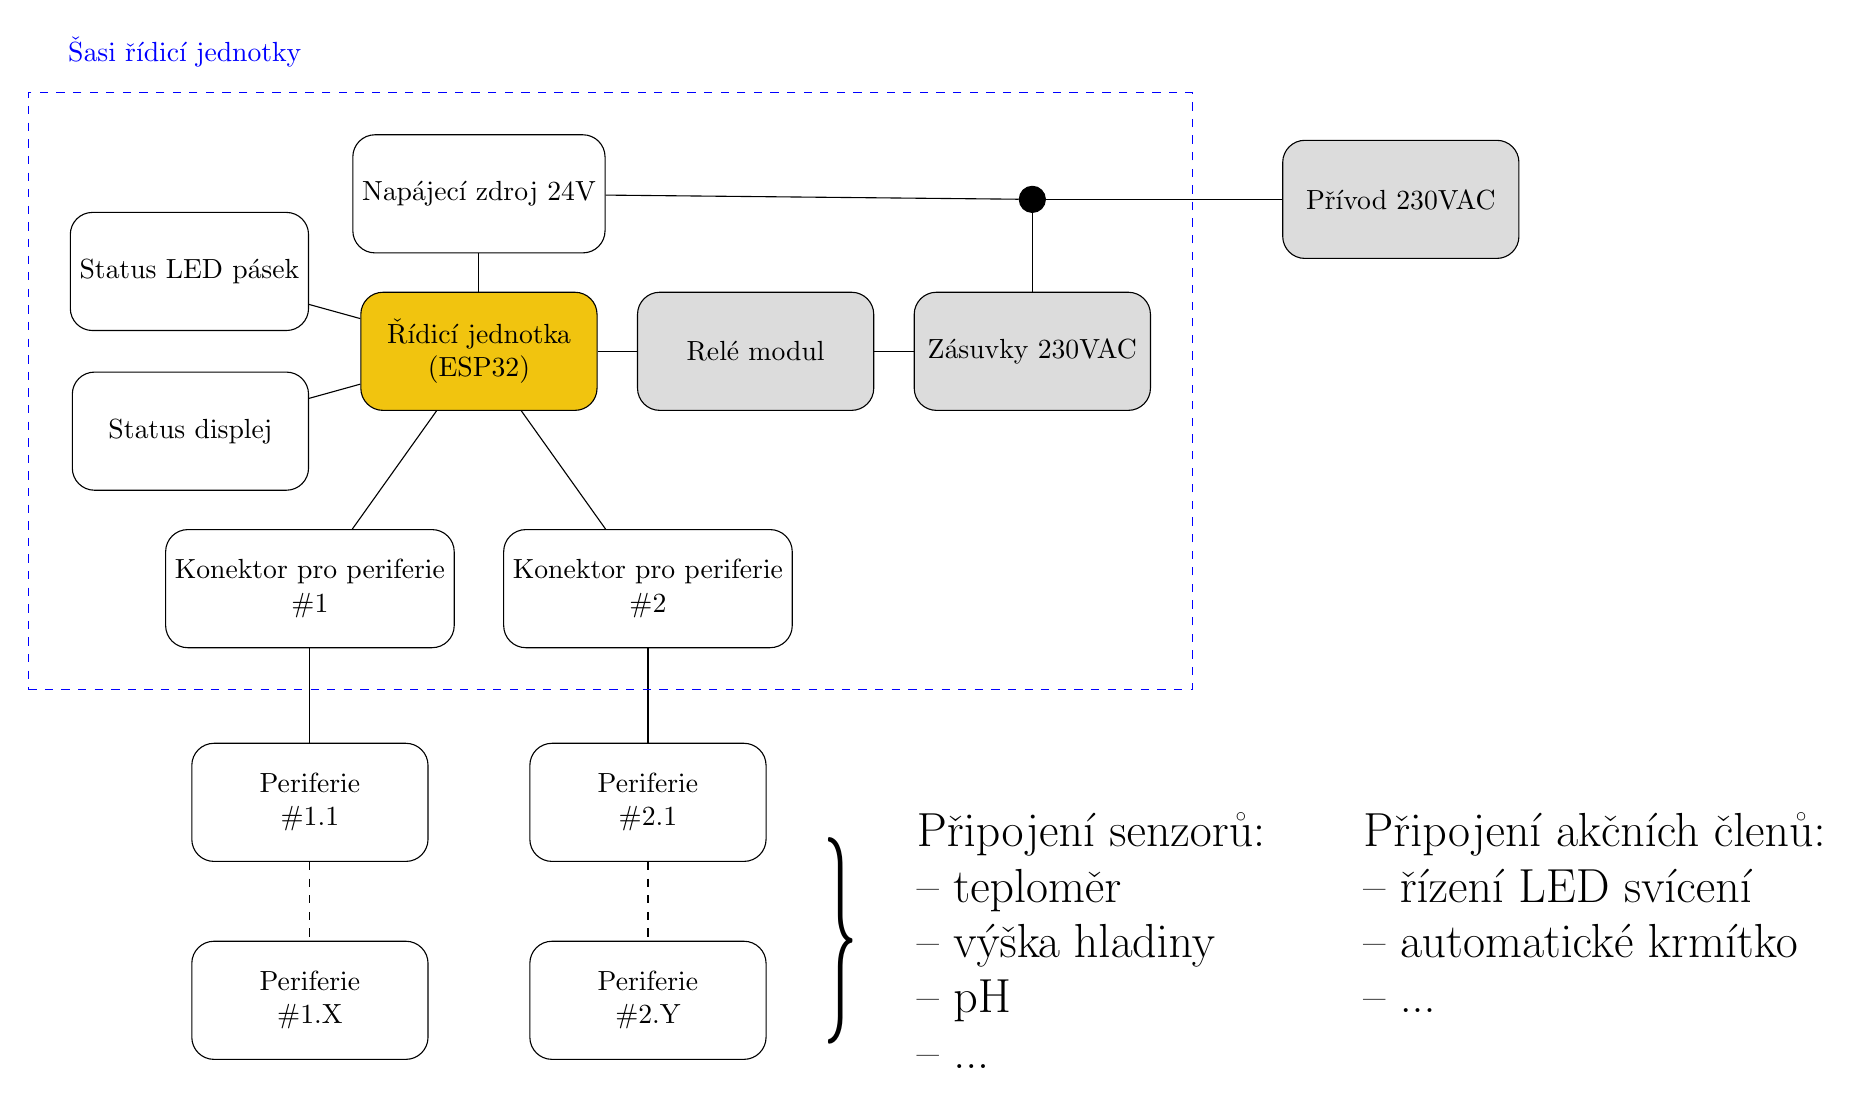
\begin{tikzpicture}[
			% scale=0.6, every node/.style={scale=0.6},
			shift={(30,30)},
			node distance=2cm,
			blok/.style={draw, rectangle, rounded corners=8pt, minimum height=1.5cm, minimum width=3cm},
			rect/.style={draw, dashed, blue, inner sep=15pt, fit={#1}},
			label/.style={blue}
		]
			% barvičky
			\definecolor{barva-silove}{RGB}{220, 220, 220}
			\definecolor{barva-ridici}{RGB}{241, 196, 15}
			% \draw (0,0) -- (4,0);
			\begin{scope}[]
				\node (napajeni) [blok, ] {Napájecí zdroj 24V};
				\node (ridici) [blok, below of = napajeni, align=center, fill=barva-ridici] {Řídicí jednotka \\ (ESP32)};
				\node (rele) [blok, right=0.5 of ridici, fill=barva-silove] {Relé modul};
				\node (zasuvky) [blok, right=0.5 of rele, fill=barva-silove] {Zásuvky 230VAC};
				\node (uzel) [style={draw, circle, minimum size=0.1cm, fill}, above=1cm of zasuvky] {};
				\node (sit) [blok, right=3 of uzel, fill=barva-silove ] {Přívod 230VAC};
				\node (display) [blok, below left=-0.5cm and 0.65cm of ridici] {Status displej};
				\node (ledstrip) [blok, above left=-0.5cm and 0.65cm of ridici] {Status LED pásek};
	
				\node (konektor1) [blok, align=center, below left=1.5cm and -1.2cm of ridici] {Konektor pro periferie \\ \#1};
				\node (konektor2) [blok, align=center, below right=1.5cm and -1.2cm of ridici] {Konektor pro periferie \\ \#2};
	
				% Periferie
				\node (per1-1) [blok, align=center, below=1.2cm of konektor1] {Periferie \\ \#1.1};
				\node (per1-x) [blok, align=center, below=1cm of per1-1] {Periferie \\ \#1.X};
			
				\node (per2-1) [blok, align=center, below=1.2cm of konektor2] {Periferie \\ \#2.1};
				\node (per2-y) [blok, align=center, below=1cm of per2-1] {Periferie \\ \#2.Y};
	
				% Popisek
				\node (vlastovka) [font=\fontsize{35}{14}\selectfont, yscale=3,  above right=-4.2cm and 0.6cm of per2-1] {\}}; 
	
				\node (popisek1) [font=\fontsize{18}{20}\selectfont,right=0.5cm of vlastovka,yshift=0cm, align=left] {Připojení senzorů: \\ -- teploměr \\ -- výška hladiny \\ -- pH \\ -- ...};
				\node (popisek2) [font=\fontsize{18}{20}\selectfont,right=1cm of popisek1.north east, anchor=north west, align=left] {Připojení akčních členů: \\ -- řízení LED svícení \\ -- automatické krmítko \\ -- ...};
				% \node (popisek3) [below=1cm of popisek2.south west, anchor=south west, align=left] {...};
	
				% Spojovací linie
				\draw[-] (sit) -- (uzel);
				\draw[-] (uzel) -- (napajeni);
				\draw[-] (uzel) -- (zasuvky);
				\draw[-] (napajeni) -- (ridici);
				\draw[-] (ridici) -- (napajeni);
				\draw[-] (ridici) -- (display);
				\draw[-] (ridici) -- (ledstrip);
				\draw[-] (ridici) -- (konektor1);
				\draw[-] (ridici) -- (konektor2);
				\draw[-] (ridici) -- (rele);
				\draw[-] (rele) -- (zasuvky);
		
				\draw[-] (konektor1) -- (per1-1);
				\draw[dashed] (per1-1) -- (per1-x);
				
				\draw[-] (konektor2) -- (per2-1);
				\draw[dashed] (per2-1) -- (per2-y);
				
			
				% Obdélník, který obklopí vybrané uzly
				\node (hlavni-cast) [rect={(napajeni) (display) (ledstrip) (konektor1) (zasuvky)}] {};
				\node[label,above left=0.2cm and -3.6cm of hlavni-cast] {Šasi řídicí jednotky};
			\end{scope}
		\end{tikzpicture}
		}
	\end{figure}
\end{frame}

%%%%%%%%%%%%%
\begin{frame}[fragile]
	\frametitle{Navržené zařízení -- prototyp}
	\vspace{-0.5cm}
	\begin{figure}%	
		% \hspace{-1.5cm}
		\includegraphics[width=1\textwidth]{obrazky/prezentace/ukazka/system-cely.jpg}
		%lze vložit popisek, ale povetšinou je to v prezentaci zbytečné
		%\caption{Popisek obrázku}%
		%\label{obr:ukazka}
	\end{figure}
\end{frame}

%%%%%%%%%%%%%
\begin{frame}[fragile]
	\frametitle{Návrh vlastního zařízení -- Řídicí jednotka}
	\vspace{-1cm}
	\begin{figure}%	
		% \hspace{-1.5cm}
		\includegraphics[width=1.05\textwidth]{obrazky/prezentace/foto-ridici.png}
		%lze vložit popisek, ale povetšinou je to v prezentaci zbytečné
		%\caption{Popisek obrázku}%
		%\label{obr:ukazka}
	\end{figure}
\end{frame}

%%%%%%%%%%%%%
\begin{frame}[fragile]
	\frametitle{Návrh vlastního zařízení -- Periferie}
		Periferie = samostatný blok připojený na sběrnici:\\[1ex]
		Univerzální modul:\\[1ex]
		%
		\begin{itemize}
			\item Vlastní MCU a regulátor napětí
			\item Komunikace po sběrnici 
			\item Napájení pro náročnější součásti (např. osvětlení)
		\end{itemize}
		\vspace{1ex}%
		%
		\begin{figure}%	
			% \hspace{-1.5cm}
			\includegraphics[width=0.95\textwidth]{obrazky/prezentace/ukazka/modul-perif.jpg}
			%lze vložit popisek, ale povetšinou je to v prezentaci zbytečné
			%\caption{Popisek obrázku}%
			%\label{obr:ukazka}
		\end{figure}


\end{frame}

%%%%%%%%%%%%%
\begin{frame}[fragile]
	\frametitle{Datová komunikace -- sběrnice  CAN}
	Tři typy zpráv:\\[1ex]
	\begin{itemize}
		\item To Slave -- požadavek řídicí jednotky
		\item To Master -- odpověď periferie
		\item Broadcast -- zpráva určená všem   
	\end{itemize}
	\vspace{2.5ex}%
	Průbeh komunikace:\\[1ex]
	\begin{itemize}
		\item Řídicí jednotka se pravidelně dotazuje periferií:
		\begin{itemize}
			\item Stav
			\item Data senzorů 
			\item Ovládání (akční členy)
		\end{itemize}
		\item Periferie pouze odpovídají na dotazy
	\end{itemize}
\end{frame}

%%%%%%%%%%%%%
\begin{frame}[fragile]
	\frametitle{Webové rozhraní}
	\vspace{-1cm}
	\begin{figure}%	
		% \hspace{-1.5cm}
		\includegraphics[width=1.05\textwidth]{obrazky/prezentace/web/hlavni-menu.jpg}
		%lze vložit popisek, ale povetšinou je to v prezentaci zbytečné
		%\caption{Popisek obrázku}%
		%\label{obr:ukazka}
	\end{figure}
\end{frame}

%%%%%%%%%%%%%
\begin{frame}[fragile]
	\frametitle{Webové rozhraní}
	\vspace{-1cm}
	\begin{figure}%	
		% \hspace{-1.5cm}
		\includegraphics[width=1.05\textwidth]{obrazky/prezentace/web/stav.jpg}
		%lze vložit popisek, ale povetšinou je to v prezentaci zbytečné
		%\caption{Popisek obrázku}%
		%\label{obr:ukazka}
	\end{figure}
\end{frame}


%%%%%%%%%%%%%
\begin{frame}[fragile]
	\frametitle{Webové rozhraní}
	\vspace{-1cm}
	\begin{figure}%	
		% \hspace{-1.5cm}
		\includegraphics[width=1.05\textwidth]{obrazky/prezentace/web/web.jpg}
		%lze vložit popisek, ale povetšinou je to v prezentaci zbytečné
		%\caption{Popisek obrázku}%
		%\label{obr:ukazka}
	\end{figure}
\end{frame}


%%%%%%%%%%%%%
\begin{frame}[fragile]
	\frametitle{Budoucí plány a rozšíření}

	\begin{columns}[T] 								% prostředí sloupce s umístěním nahoře
		\begin{column}{0.5\textwidth}		% první sloupec
			\begin{block}{Blízká budoucnost}
				\begin{itemize}
					\item Oprava nalezených chyb
					\item Praktická aplikace v akváriu
					\item Přidání grafického displeje
					\item Výroba dalších periferií
				\end{itemize}
			\end{block}
		\end{column}
		%
		\begin{column}{0.5\textwidth}		% druhý sloupec
			\begin{alertblock}{Vzdálená budoucnost}
				\begin{itemize}
					\item Modifikace pro další oblasti domácí automatizace

				\end{itemize}
			\end{alertblock}
		\end{column}
	\end{columns}											% ukončení prostředí sloupce
\end{frame}



% podekovani
\begin{frame}[c] 
% bez nadpisu snímku
	\frametitle{\mbox{ }}
	\begin{center}
		{\Huge Děkuji za pozornost!}
	\end{center}
\end{frame}

% otázky oponenta
\begin{frame}[fragile] 
\frametitle{Otázky oponenta}
	\emph{Stanovte maximální provozní spotřebu všech periferií napájených LDO a stanovte jeho ztrátový výkon. Tyto údaje vám v bakalářské práci chybí.}\\[0.5ex]
	%
	\begin{figure}%	
		\centering
		\scalebox{0.9}
		{
			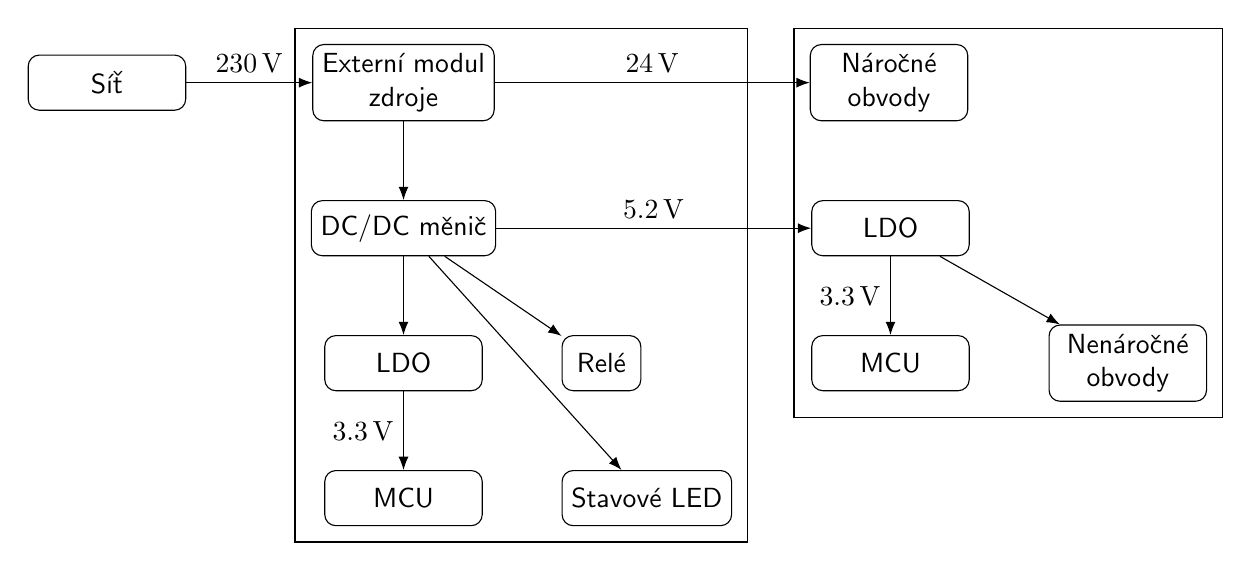
\begin{tikzpicture}[
				module/.style={%
			draw, rounded corners,
			minimum width=#1,
			minimum height=7mm,
			font=\sffamily,
			align=center
			},
		module/.default=2cm,
		>=LaTeX]
			
		% ridici
		\node[module] (24v) {Externí modul\\zdroje};
		\node[module, left=1.6cm of 24v] (sit) {Síť};
		\node[module, below=of 24v] (buck) {DC/DC měnič};
		\node[module, below=of buck] (ldo) {LDO}; 
		\node[module, below=of ldo] (mcu) {MCU};

		\node[module, right= of mcu] (konektor1) {Stavové LED};
		\node[module=1cm, right=of ldo] (konektor3) {Relé};

		\node[fit=(konektor1) (24v) (konektor3) (buck) (mcu), draw, inner sep=2mm] (fitridici) {};

		\node[module, right= 4cm of buck] (ldoperif) {LDO};
		\node[module, below=of ldoperif] (mcuperif) {MCU};
		\node[module, right= 4cm of 24v] (naro) {Náročné\\obvody};
		\node[module, right=of mcuperif] (nenaro) {Nenáročné\\obvody};

		\node[fit=(ldoperif) (mcuperif) (nenaro) (naro), draw, inner sep=2mm] (fitperif) {};


		% % Connections
		\draw[->] (sit)--(24v) node[midway, above] {\qty{230}{V}};		
		\draw[->] (24v)--(buck);
		\draw[->] (24v)--(naro) node[midway, above] {\qty{24}{V}};
		\draw[->] (buck)--(ldo);
		\draw[->] (buck)--(konektor1);
		\draw[->] (buck)--(konektor3);
		\draw[->] (ldo)--(mcu) node[midway, left] {\qty{3.3}{V}};
		\draw[->] (buck)--(ldoperif) node[midway, above] {\qty{5.2}{V}};
		\draw[->] (ldoperif)--(mcuperif) node[midway, left] {\qty{3.3}{V}};
		\draw[->] (ldoperif)--(nenaro);
			
		\end{tikzpicture}
		}
	\end{figure}
\end{frame}

% otázky oponenta
\begin{frame}[fragile] 
	\frametitle{Otázky oponenta}
	Řídicí jednotka:
	\begin{itemize}
		\item MCU: \(I_{TXpeak}= \qty{379}{mA}\), \(I_{TXavg}= \qty{239}{mA}\)
		\item CAN řadič: \(I_{IO_rdom}=\qty{500}{\micro A} \) 
	\end{itemize}
	\vspace{1cm}
	\begin{equation}
		I_{MAX} = \qty{379}{mA}+\qty{500}{\micro A} = \qty{379.5}{mA}
	\end{equation}
	\vspace{0.5cm}
		\begin{equation}
			P_{LDO} = (U_{IN} - U_{OUT})\cdot I_{MAX} = (\qty{5.2}{V} - \qty{3.3}{V})\cdot \qty{379.5}{mA} = \qty{721}{mW}
		\end{equation}
	\end{frame}

	% otázky oponenta
\begin{frame}[fragile] 
	\frametitle{Otázky oponenta}
	Periferie:
	\begin{itemize}
		\item MCU: \(I_{Vdd-max}= \qty{85}{mA}\)
		\item CAN řadič: \(I_{IO_rdom}=\qty{500}{\micro A} \) 
		\item Teplotní čidlo: \(I_{ds18b20} =\qty{1.5}{mA}\) 
	\end{itemize}
	\vspace{1cm}
	\begin{equation}
		I_{MAX} = \qty{85}{mA}+\qty{500}{\micro A}+\qty{1.5}{mA} = \qty{87}{mA}
	\end{equation}
	\vspace{0.5cm}
		\begin{equation}
			P_{LDO} = (U_{IN} - U_{OUT})\cdot I_{MAX} = (\qty{5.2}{V} - \qty{3.3}{V})\cdot \qty{87}{mA} = \qty{165}{mW}
		\end{equation}
	\end{frame}

% zdroje
\begin{frame} [fragile]
	% bez nadpisu snímku
	\frametitle{Zdroje obrázků}
	% \hspace{-5cm}
	\begin{itemize}
		\item \url{https://www.reef2reef.com/threads/lets-see-your-ghl.258905/#post-3069873}
		\item \url{https://brushknight.medium.com/terrarium-controller-idea-%EF%B8%8F-v1-4-b8ee96cfbd22}
		\item \url{https://www.pyramidions.com/blog/the-advantages-of-using-the-cloud-technology-for-app-development/}
		\item \url{https://www.flaticon.com/free-icons/money}
		\item \url{https://www.flaticon.com/free-icons/shock}
	\end{itemize}			
\end{frame}

%%%%%%%%%%%%%
\begin{frame}[fragile]
	\frametitle{Připojení periferií}
	
			Požadavky periferií:\\[1ex]
			%
			\begin{itemize}
				\item Napájení vlastního MCU
				\item Datová komunikace 
				\item Napájení výkonově náročnějších součástí (např. osvětlení)
			\end{itemize}
			\vspace{1.5ex}%
		%
		Konektor D-sub:\\[1ex]
		\begin{figure}[h!]
			\centering
			% trim=left bottom right top
			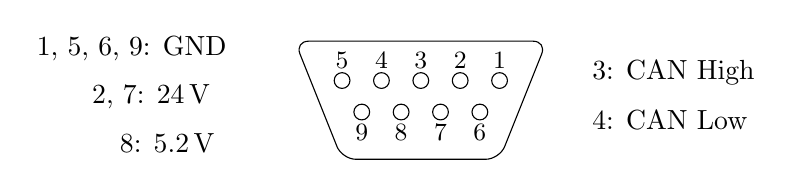
\begin{tikzpicture}
	
				% Draw the connector outline
				\draw[rounded corners=5pt] (0,0) -- (2,0) -- (2.6,1.5) -- (-0.6,1.5) -- cycle;
				
				% Draw the pins
				\newcounter{pinnum}
				\setcounter{pinnum}{9}
				\def\xoff{-0.25}
				\foreach \x in {0.5,1,...,2}
					\foreach \y in {0.6}
					{
						\draw (\xoff+\x,\y) circle (0.1);
						\node[anchor=north,font=\fontsize{9}{0}\selectfont] at (\xoff+\x,\y-0.03) {\thepinnum};
						\setcounter{pinnum}{\value{pinnum}-1}
					}
	
				\def\xoff{-0.5}
				\foreach \x in {0.5,1,...,2.5}
					\foreach \y in {1.0}
					{
						\draw (\xoff+\x,\y) circle (0.1);
						\node[anchor=south,font=\fontsize{9}{0}\selectfont] at (\xoff+\x,\y+0.03) {\thepinnum};
						\setcounter{pinnum}{\value{pinnum}-1}
					}
				
				% Pin numbers
				\node[anchor=west] (pin1) at (-4,1.4)                            {1,~5,~6,~9: GND};
				\node[below=0.6 of pin1.west,anchor=west] (pin2) {~~~~~~2,~7: \qty{24}{V}};
				\node[below=0.6 of pin2.west,anchor=west] (pin3) {~~~~~~~~~8: \qty{5.2}{V}};
				\node[anchor=west] at (2,1.1) (pin4) {~~~~~~~~~3: CAN High};
				\node[below=0.6 of pin4.west,anchor=west] (pin5) {~~~~~~~~~4: CAN Low};
				
			\end{tikzpicture}
		\end{figure}
\end{frame}



%%%%%%%%%%%%%
\begin{frame}[fragile]
	\frametitle{Blokové schéma -- Řídicí jednotka}
	\vspace{-0.7cm}
	\begin{figure}%	
		\centering
		\scalebox{0.9}
		{
			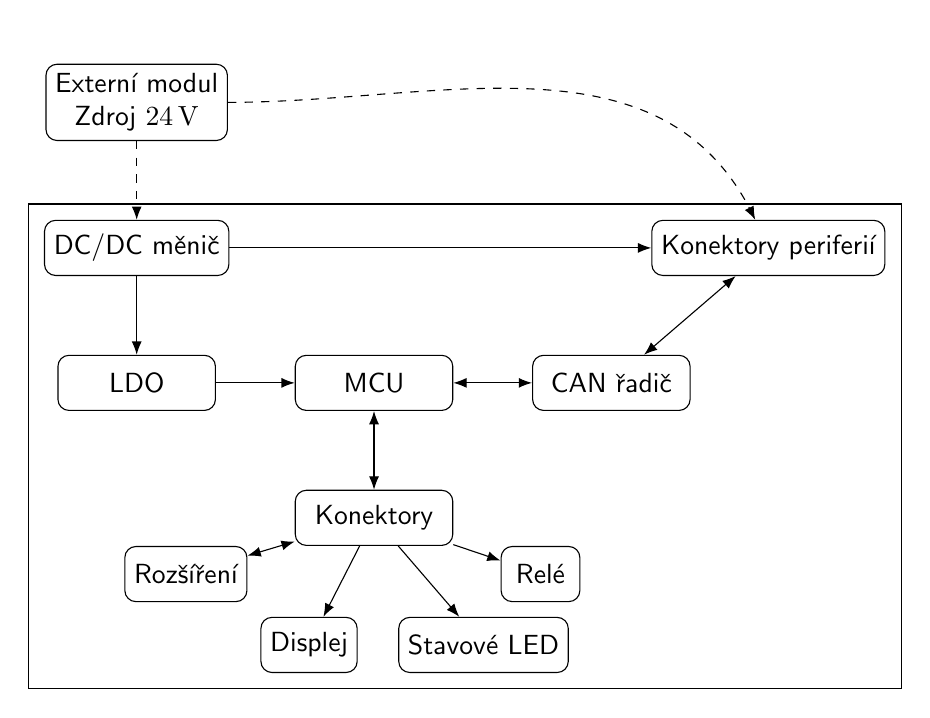
\begin{tikzpicture}[
				module/.style={%
			draw, rounded corners,
			minimum width=#1,
			minimum height=7mm,
			font=\sffamily,
			align=center
			},
		module/.default=2cm,
		>=LaTeX]
			
				% ridici
				\node[module] (mcu) {MCU};
				\node[module, left=of mcu] (ldo) {LDO}; 
				\node[module, above=of ldo] (buck) {DC/DC měnič};
				\node[module, right=of mcu] (candriver) {CAN řadič};
				\node[module, above right=10mm and -5mm of candriver] (konperif) {Konektory periferií};
				\node[module, above=of buck] (24v) {Externí modul\\Zdroj \qty{24}{V}};
				\node[module, below=of mcu] (konektory) {Konektory};
				\node[module=1cm, below right=9mm and -7mm of konektory] (konektor1) {Stavové LED};
				\node[module=1cm, below left= 9mm and -8mm of konektory] (konektor2) {Displej};
				\node[module=1cm, below right= 0mm and 6mm of konektory] (konektor3) {Relé};
				\node[module=1cm, below left= 0mm and 6mm of konektory] (konektor4) {Rozšíření};
	
				\node[fit=(konektor1) (konektor2) (konektor3) (konektor4) (buck) (konperif) (mcu), draw, inner sep=2mm] (fitridici) {};
				% Connections
				\foreach \i in {1,2,3}
					\draw[->] (konektory)--(konektor\i);
				\draw[<->] (konektory)--(konektor4);
				\draw[<->] (konektory)--(mcu);
				\draw[->] (buck)--(ldo);
				\draw[->] (ldo)--(mcu);
				\draw[<->] (candriver)--(mcu);
				\draw[->] (buck)--(konperif);
				\draw[<->] (candriver)--(konperif);
	
				\draw[->,dashed] (24v) to [out=0,in=115] (konperif);
				\draw[->,dashed] (24v)--(buck);
			
			\end{tikzpicture}
		}
	\end{figure}
\end{frame}

%%%%%%%%%%%%%
\begin{frame}[fragile]
	\frametitle{Blokové schéma -- Software}
	\vspace{-0.65cm}
	\begin{figure}%	
		\centering
		\scalebox{0.7}
		{
			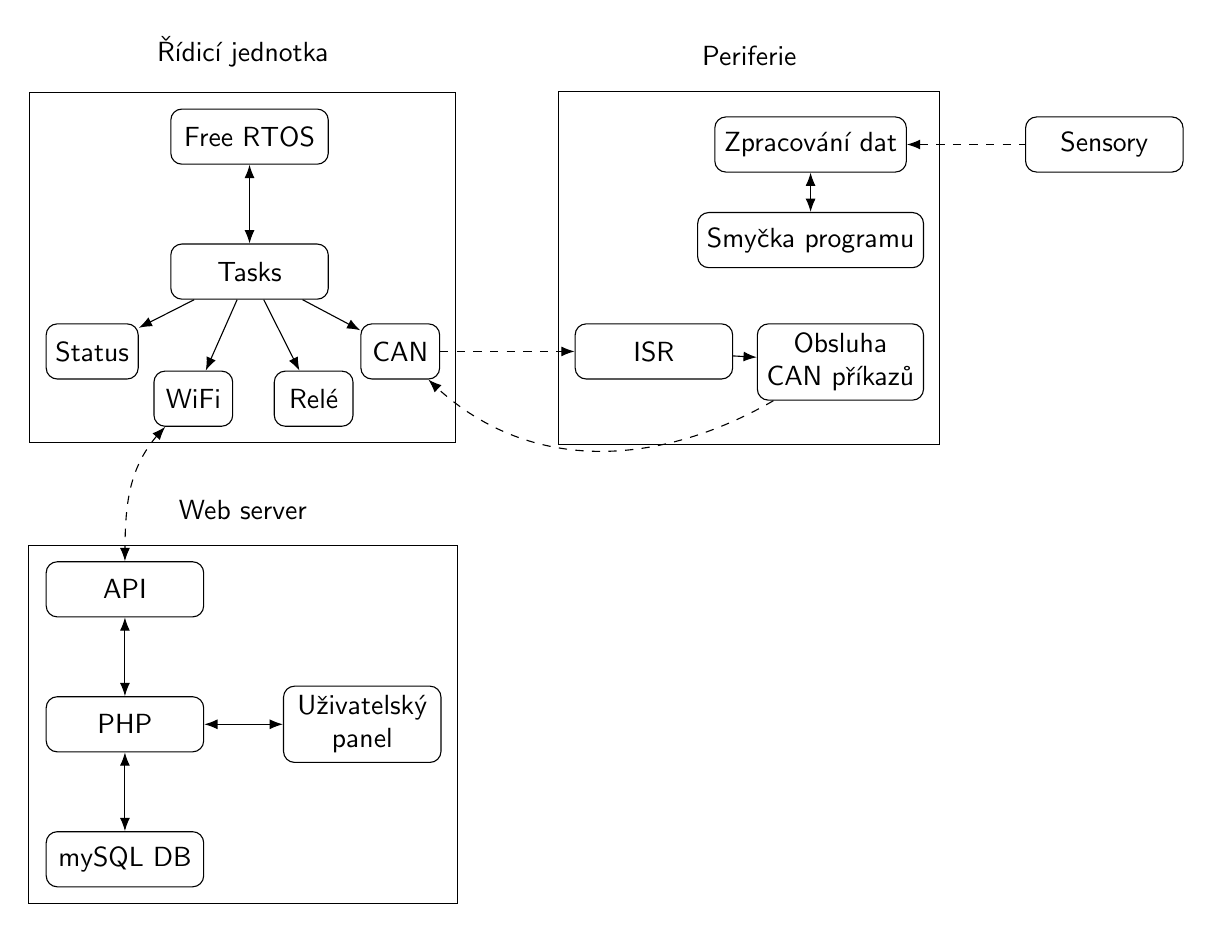
\begin{tikzpicture}[
				module/.style={%
			draw, rounded corners,
			minimum width=#1,
			minimum height=7mm,
			font=\sffamily,
			align=center
			},
		module/.default=2cm,
		>=LaTeX]
			
				% ridici
				\node[module] (freertos) {Free RTOS};
				\node[module, below=of freertos] (tasks) {Tasks};
				\node[module=1cm, below right=9mm and -7mm of tasks] (task1) {Relé};
				\node[module=1cm, below left= 9mm and -8mm of tasks] (task2) {WiFi};
				\node[module=1cm, below right= 3mm and 4mm of tasks] (task3) {CAN};
				\node[module=1cm, below left= 3mm and 4mm of tasks] (task4) {Status};
	
				\node[fit=(task1) (task2) (task3) (task4) (freertos), draw, inner sep=2mm,label={[yshift=2mm, font=\sffamily]Řídicí jednotka}] (fitridici) {};
				% Connections
				\foreach \i in {1,2,3,4}
					\draw[->] (tasks)--(task\i);
				\draw[<->] (tasks)--(freertos);
	
				% WS
				\node[module, below=1.5cm of {task4.west|-fitridici.south}, anchor=north west] (api) {API};
				\node[module, below=of api] (php) {PHP};
				\node[module, below=of php] (mysql) {mySQL DB};
				\node[module, right= of php] (userweb) {Uživatelský \\panel};
				\node[fit={(php) (userweb) (api) (mysql) (mysql-|fitridici.west) (mysql-|fitridici.east) }, draw, inner xsep=\pgflinewidth, inner ysep=2mm, label={[yshift=2mm, font=\sffamily]Web server}] (fitWS) {};
				\draw[<->] (api)--(php);
				\draw[<->] (php)--(mysql);
				\draw[<->] (php)--(userweb);
			
				% perif
				\node[module, right=1.5cm of {task3-|fitridici.east}] (isr) {ISR};
				\node[module, right=3mm of isr.north east, anchor=north west] (can) {Obsluha\\CAN příkazů};
				\node[module, above= 7mm of can.north east, anchor=south east] 
					(programloop) {Smyčka programu};
				\node[module, above=5mm of programloop] (dataprocess) {Zpracování dat};
				
				\node[fit={(can) (isr) (dataprocess|-fitridici.south) (dataprocess|-fitridici.north)}, draw, inner xsep=2mm, inner ysep=\pgflinewidth, label={[yshift=2mm, font=\sffamily]Periferie}] (fitperif) {};
				\node[module, right=1.5cm of dataprocess] (sensory) {Sensory};
				\draw[->] (isr)--(can);
				\draw[<->] (programloop)--(dataprocess);
				
				%arrow between boxes
				\draw[<->,dashed] (task2) to [out=-135,in=90] (api);
				\draw[->,dashed] (task3)--(isr);
				\draw[->,dashed] (can) to [out=-150,in=-45] (task3);
				\draw[<-,dashed] (dataprocess) -- (sensory);
			\end{tikzpicture}
		}
	\end{figure}
\end{frame}

%%%%%%%%%%%%%
\begin{frame}[fragile]
	\frametitle{Stavové LED řídicí jednotky}
	\vspace{-0.65cm}
	\begin{figure}%	
		\centering
		\scalebox{0.8}
		{
			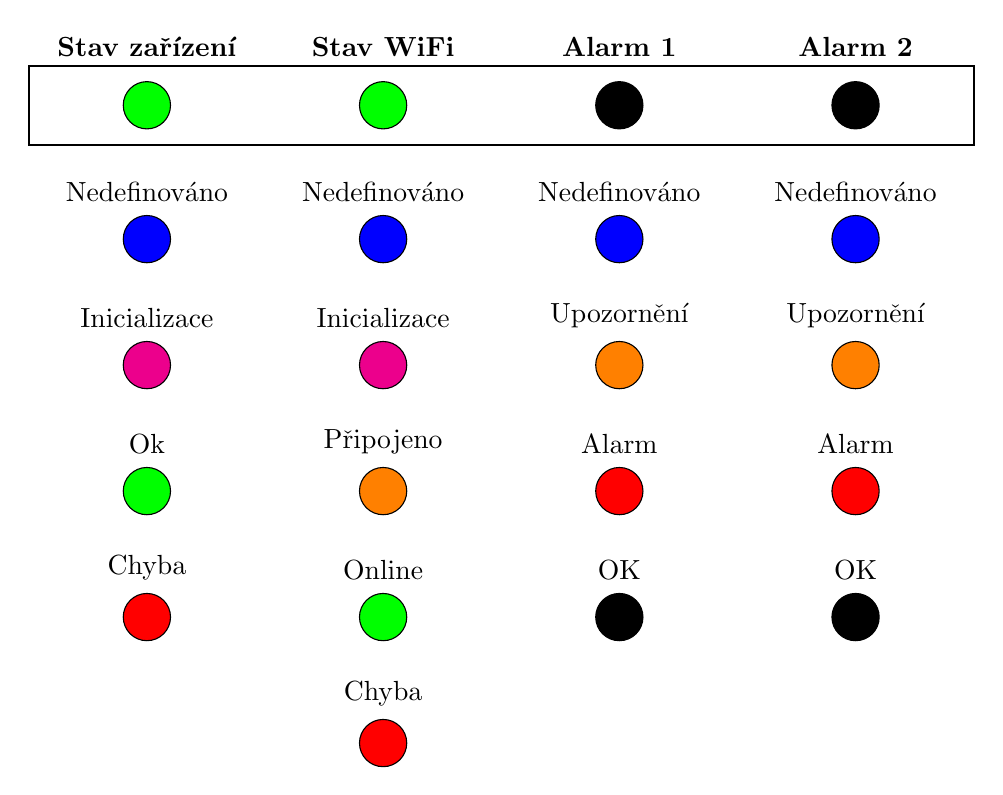
\begin{tikzpicture}
                % Draw a rectangle
                \draw[thick] (0,0) rectangle (3*4,1);
                
                % Draw and fill four colorful circles
                \filldraw[fill=green,draw=black,thin]  (3*0.5, 0.5) circle (0.3) node[align=center,above=0.5] {\textbf{Stav zařízení}};
                \filldraw[fill=green,draw=black,thin]  (3*1.5, 0.5) circle (0.3) node[align=center,above=0.5] {\textbf{Stav WiFi}};
                \filldraw[fill=black,draw=black,thin]  (3*2.5, 0.5) circle (0.3) node[align=center,above=0.5] {\textbf{Alarm 1}};
                \filldraw[fill=black,draw=black,thin]  (3*3.5, 0.5) circle (0.3) node[align=center,above=0.5] {\textbf{Alarm 2}};

                % Draw and fill four colorful circles
                \filldraw[fill=blue,draw=black,thin]    (3*0.5, -1.5*0.8) circle (0.3) node[align=center,above=0.35] {Nedefinováno};
                \filldraw[fill=blue,draw=black,thin]    (3*1.5, -1.5*0.8) circle (0.3) node[align=center,above=0.35] {Nedefinováno};
                \filldraw[fill=blue,draw=black,thin]    (3*2.5, -1.5*0.8) circle (0.3) node[align=center,above=0.35] {Nedefinováno};
                \filldraw[fill=blue,draw=black,thin]  (3*3.5, -1.5*0.8) circle (0.3) node[align=center,above=0.35] {Nedefinováno};

                % Draw and fill four colorful circles
                \filldraw[fill=magenta,draw=black,thin] (3*0.5, -3.5*0.8) circle (0.3) node[align=center,above=0.35] {Inicializace};
                \filldraw[fill=magenta,draw=black,thin] (3*1.5, -3.5*0.8) circle (0.3) node[align=center,above=0.35] {Inicializace};
                \filldraw[fill=orange,draw=black,thin]  (3*2.5, -3.5*0.8) circle (0.3) node[align=center,above=0.35] {Upozornění};
                \filldraw[fill=orange,draw=black,thin]  (3*3.5, -3.5*0.8) circle (0.3) node[align=center,above=0.35] {Upozornění};

                % Draw and fill four colorful circles
                \filldraw[fill=green,draw=black,thin]   (3*0.5, -5.5*0.8) circle (0.3) node[align=center,above=0.35] {Ok};
                \filldraw[fill=orange,draw=black,thin]  (3*1.5, -5.5*0.8) circle (0.3) node[align=center,above=0.35] {Připojeno};
                \filldraw[fill=red,draw=black,thin]   (3*2.5, -5.5*0.8) circle (0.3) node[align=center,above=0.35] {Alarm};
                \filldraw[fill=red,draw=black,thin]  (3*3.5, -5.5*0.8) circle (0.3) node[align=center,above=0.35] {Alarm};

                % Draw and fill four colorful circles
                \filldraw[fill=red,draw=black,thin]     (3*0.5, -7.5*0.8) circle (0.3) node[align=center,above=0.35] {Chyba};
                \filldraw[fill=green,draw=black,thin]   (3*1.5, -7.5*0.8) circle (0.3) node[align=center,above=0.35] {Online};
                \filldraw[fill=black,draw=black,thin]   (3*2.5, -7.5*0.8) circle (0.3) node[align=center,above=0.35] {OK};
                \filldraw[fill=black,draw=black,thin]   (3*3.5, -7.5*0.8) circle (0.3) node[align=center,above=0.35] {OK};

                % Draw and fill four colorful circles
                \filldraw[fill=red,draw=black,thin]     (3*1.5, -9.5*0.8) circle (0.3) node[align=center,above=0.35] {Chyba};
            \end{tikzpicture}
		}
	\end{figure}
\end{frame}


%%%%%%%%%%%%%
\begin{frame} 
	\frametitle{Vybavení akvária}
	
	\begin{columns}[T] 								% prostředí sloupce s umístěním nahoře
		\begin{column}{0.4\textwidth}		% první sloupec
			Požadavky jsou určeny:\\[0ex]
			%
			\begin{itemize}
				\item Velikostí nádrže
				\item Výběrem osazenstva 
				\item Slaná / sladká voda 
			\end{itemize}

			\vspace{2ex}%
			Základní technika:\\[0ex]
			%
			\begin{itemize}
				\item Filtr vody
				\item Topné těleso
				\item Osvětlení 
				\item Senzory
			\end{itemize}
		\end{column}
		%
		\begin{column}{0.6\textwidth}		% druhý sloupec
			\begin{figure}%	
				\centering
				% \vspace{1cm}	              % horizontální mezera
				\includegraphics[width=\columnwidth]{obrazky/prezentace/vybaveni-akvaria/06-sensory.png}
				%lze vložit popisek, ale povetšinou je to v prezentaci zbytečné
				%\caption{Popisek obrázku}%
				%\label{obr:ukazka}
			\end{figure}
		\end{column}
	\end{columns}											% ukončení prostředí sloupce
\end{frame}

\end{document}
